\chapter{Diseño}

\section{Introducción}
En este capítulo se realizará el diseño del software a desarrollar. Para ello, se detallará cómo se va a desarrollar la aplicación, qué arquitectura y tecnologías se van a utilizar y cómo se va a realizar el diseño de la interfaz de usuario. 
Esta fase tiene como objetivo definir la estructura del sistema y la función de cada una de sus partes, lo cual permitirá que el desarrollo sea más eficiente y que el resultado final tenga mayor calidad.

\subsection{Arquitectura del sistema}
Para el desarrollo de la aplicación se ha decidido utilizar una arquitectura \textbf{cliente-servidor}, donde el servidor será responsable de las operaciones relacionadas con la gestión (añadir, extraer, eliminar y/o modificar) de la información almacenada en la base de datos, mientras que el cliente será 
la aplicación móvil que se encargará de mostrar la información al usuario y de realizar las operaciones que el usuario solicite. Además, también será una arquitectura basada en el patrón de diseño \textbf{Modelo / Vista / Controlador (MVC)}, donde el modelo gestionará y mantendrá la estructura de la información
de la base de datos, la vista se hará cargo de mostrar la información al usuario y facilitar la interacción de este con el sistema y el controlador se encargará de gestionar las operaciones que el usuario solicite. Todo esto mediante las tecnologías \textbf{Node.js} para el controlador,  \textbf{MongoDB} (y mongoose) para
el modelo y \textbf{Flutter} para las distintas vistas que los usuarios tendrán. 

\begin{figure}[H]
    \centering
    \centerline{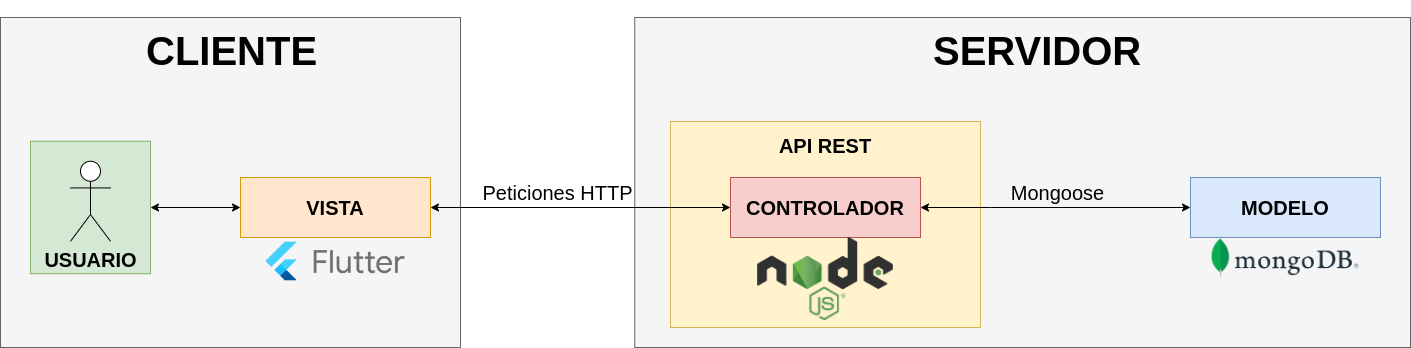
\includegraphics[width=\textwidth]{imagenes/c6/arch.png}}
    \caption{Diagrama de la arquitectura del sistema, donde se muestra la comunicación entre el servidor y la aplicación móvil.}
    \label{fig:diagramadearquitectura}    
\end{figure}

\subsection{Diagrama de base de datos}
En cuanto al diagrama de base de datos, se ha realizado un diagrama de base de datos no relacional, que representa los distintos documentos 
que tendrá nuestra base de datos de MongoDB. En este caso, se han definido 5 documentos, uno para los usuarios, otro para las lecciones, otro para los tests, otro para las preguntas de los tests y otro para
los logros. También se han definido las referencias que habrá entre los documentos, como por ejemplo que un usuario tiene varios logros.

\begin{figure}[H]
    \centering
    \centerline{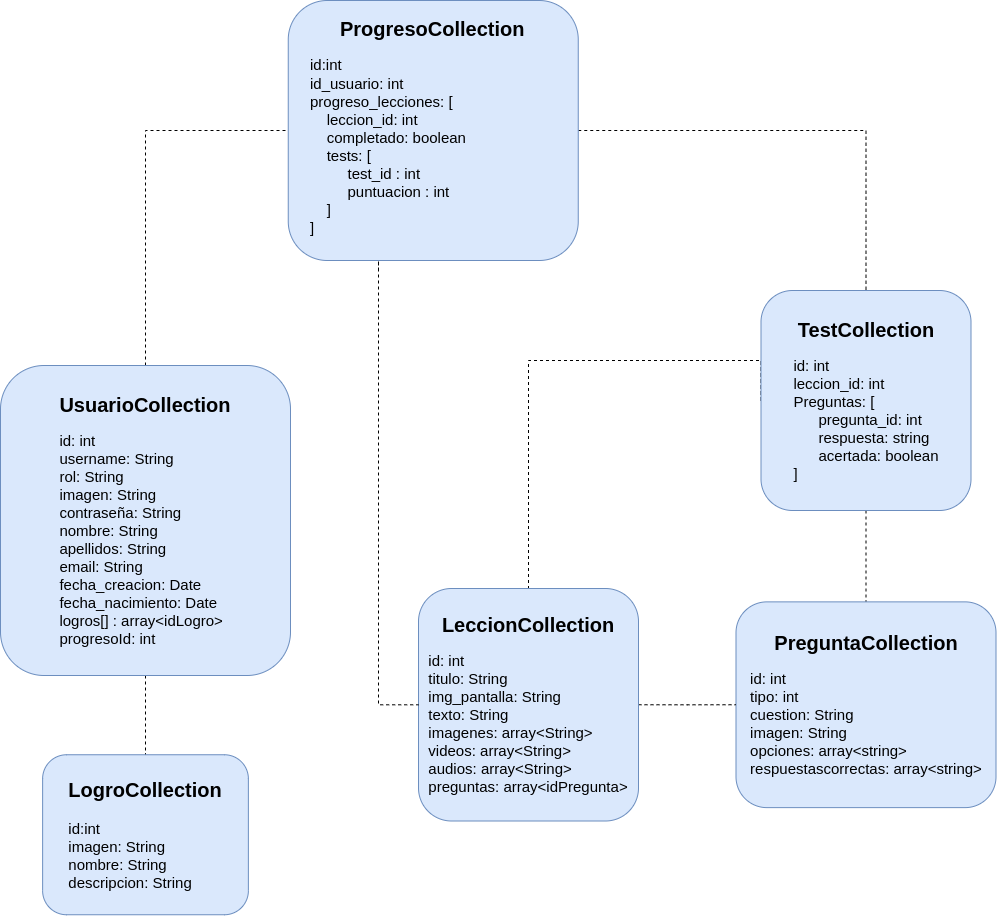
\includegraphics[width=\textwidth]{imagenes/c6/bbdd.png}}
    \caption{Diagrama de base de datos del sistema, donde se muestran los documentos que se van a almacenar en nuestra base de datos de MongoDB.}
    \label{fig:diagramadearquitectura}    
\end{figure}


\subsection{Diagrama de clases}
A continuación se muestra el diagrama de clases de diseño, el cual se ha realizado a partir del diagrama de clases de análisis del capítulo anterior En esta ocasión se han detallado más
los atributos y los métodos de cada clase, facilitando así la comprensión de las relaciones entre las clases y de la estructura del sistema.
\begin{figure}[H]
    \centering
    \centerline{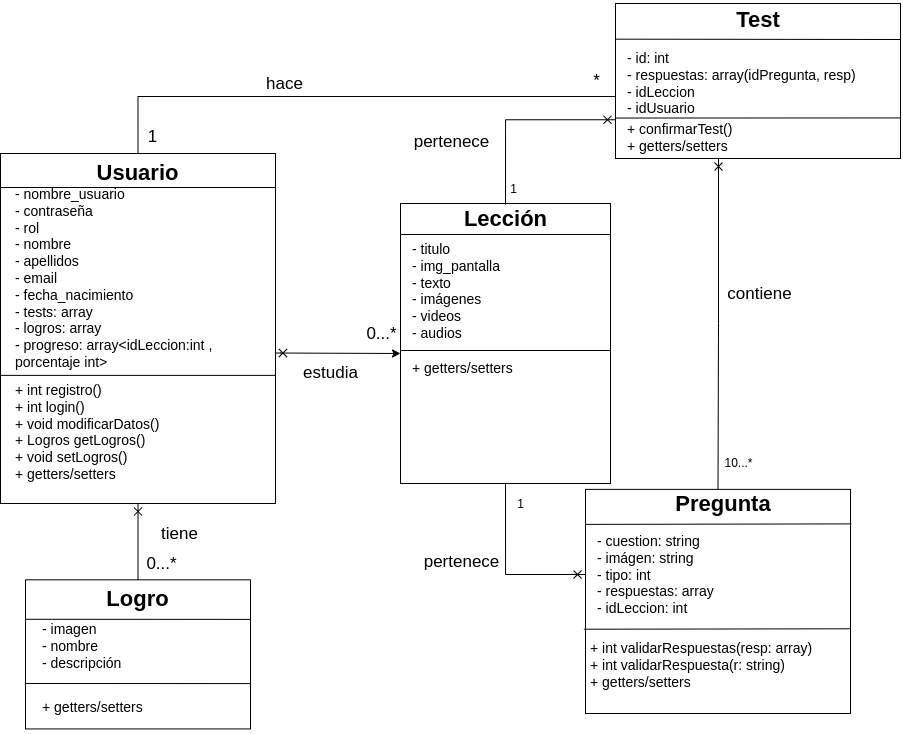
\includegraphics[width=\textwidth]{imagenes/c6/diagramadeclases.png}}
    \caption{Diagrama de clases del sistema donde se detallan las propiedades y las relaciones de las distintas clases o entidades que tendrá el software.}
    \label{fig:diagramadearquitectura}    
\end{figure}

\subsection{Diagramas de secuencia}
En lo que respecta a los diagramas de secuencia, se han realizado algunos ejemplos de cómo sería el flujo de una operación en el sistema. Como hemos visto anteriormente,
se seguirá una arquitectura basada en el patrón de diseño MVC, por lo que las peticiones pasarán por la vista, luego por el controlador y finalmente por el modelo.
En este caso, se ha realizado un diagrama de secuencia de cómo sería el flujo de una operación en la que un usuario se registra en la aplicación, otro para un usuario que contesta un test y otro
para un profesor que modifica una lección.

\begin{figure}[H]
    \centering
    \centerline{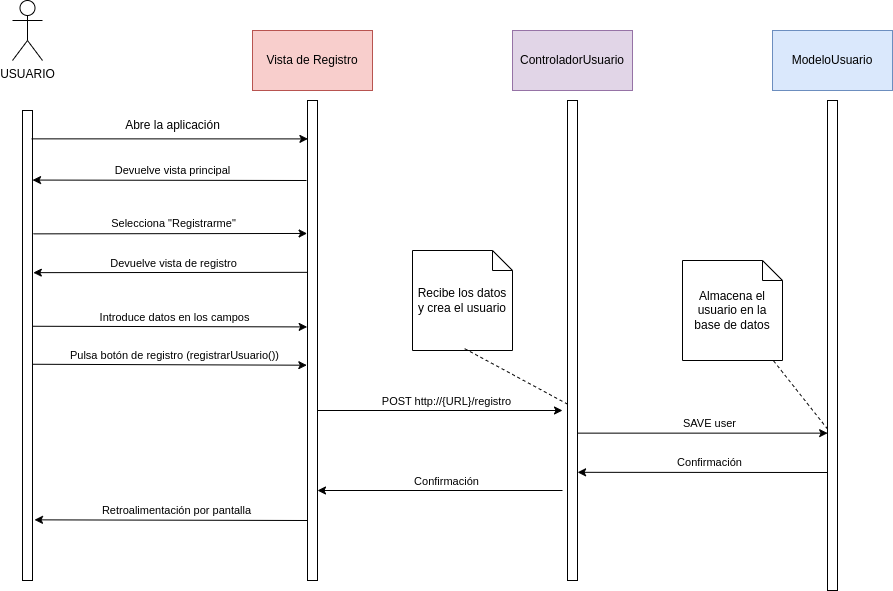
\includegraphics[width=\textwidth]{imagenes/c6/diagramadesecuencia.png}}
    \caption{Diagrama de secuencia de un usuario registrandose, el cual interactuará con la vista para poder hacer la petición al controlador y guardar su usuario en el modelo.}
    \label{fig:diagramadesecuencia}    
\end{figure}


\subsection{Diseño de interfaces de usuario}
Por último, en este apartado se presentan los bocetos de las interfaces de usuario que se han diseñado para la aplicación. Estos bocetos se han realizado con la herramienta Canva y serán de ayuda para la realización del diseño final de las interfaces de usuario,
que, pese a que seguirán una estructura similar a la de los bocetos, podrán variar en algunos detalles y aspectos de diseño.

\begin{figure}[H]
    \centering
    \centerline{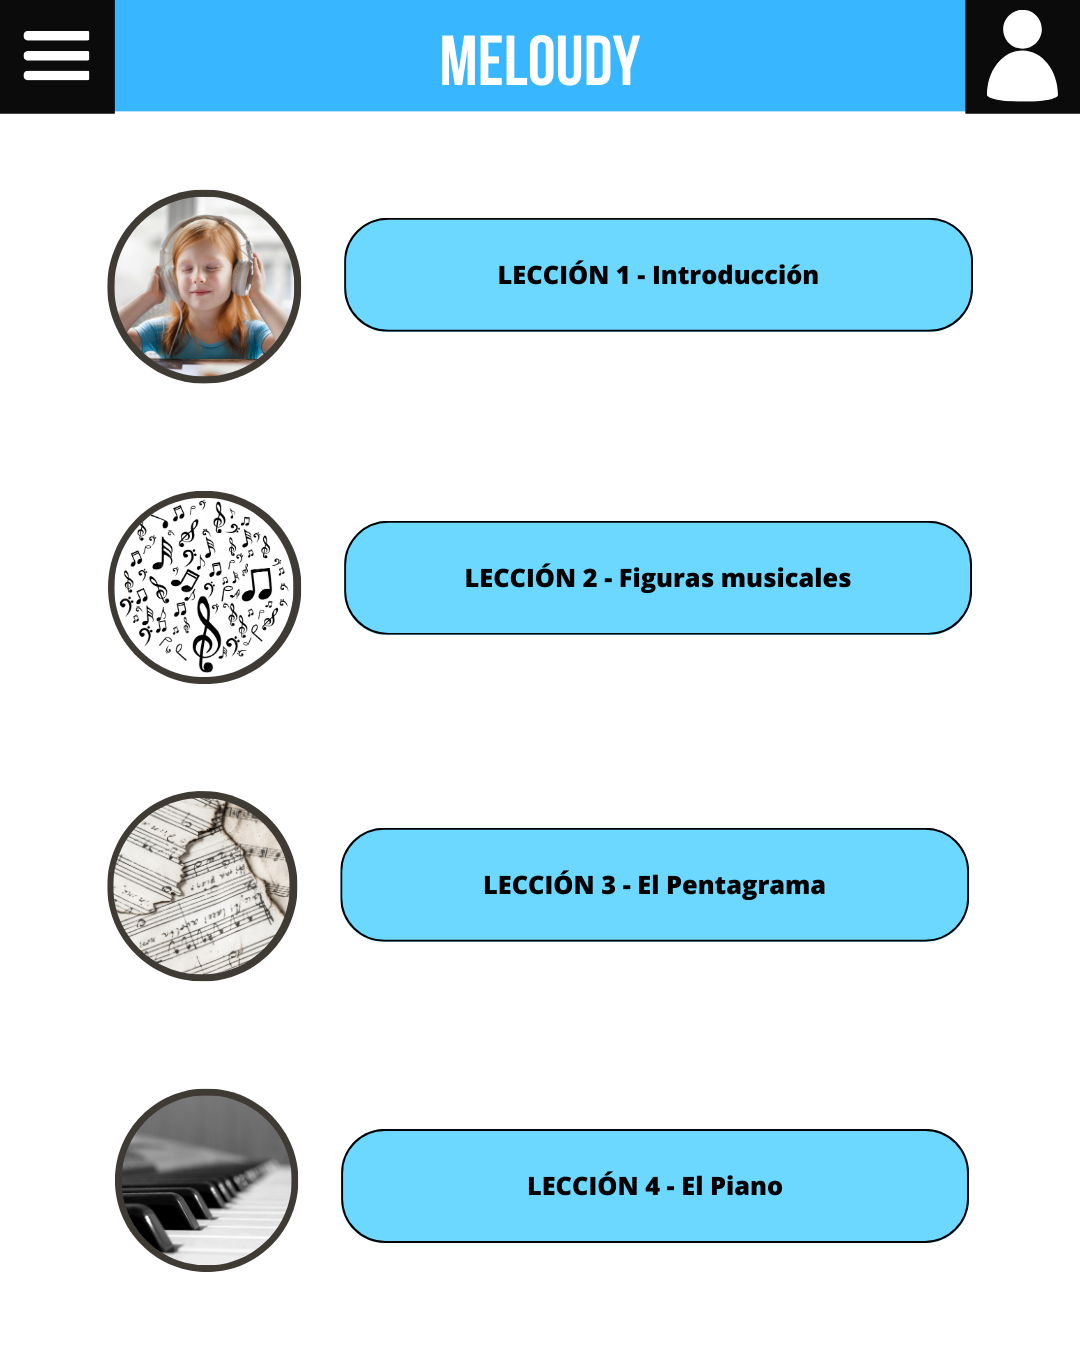
\includegraphics[width=0.55\textwidth, frame]{imagenes/c6/1.png}}
    \caption{Boceto de la pantalla principal de la aplicación donde se muestran las lecciones disponibles para el usuario.}
    \label{fig:pantallaprincipal}
    
    
\end{figure}

\begin{figure}[H]
    \centering
    \centerline{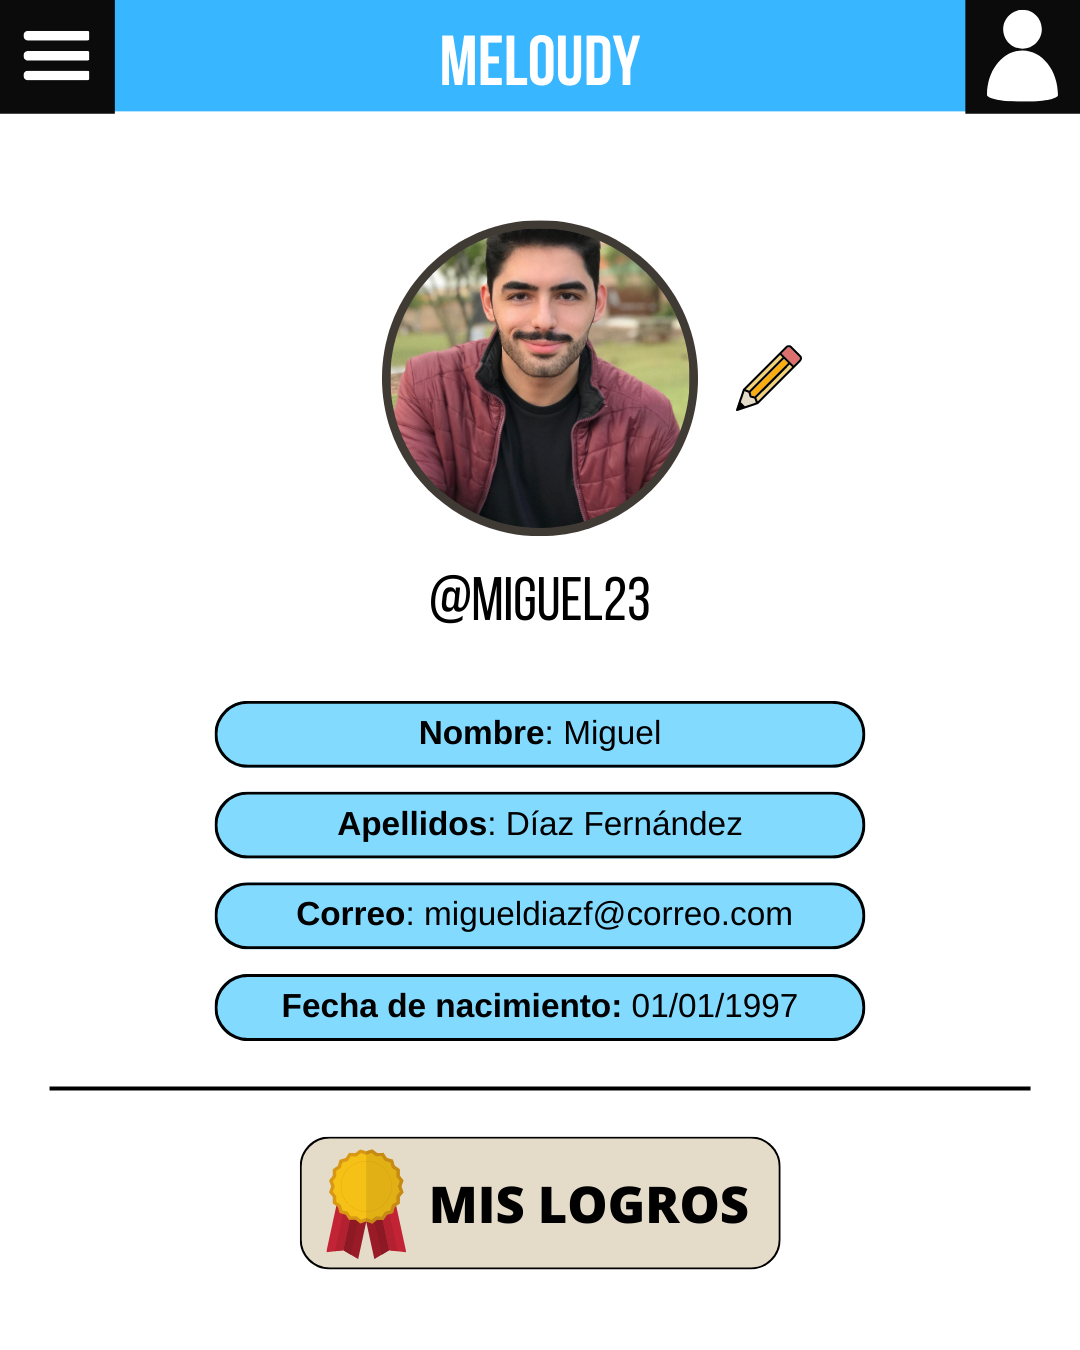
\includegraphics[width=0.55\textwidth, frame]{imagenes/c6/2.png}}
    \caption{Boceto de la pantalla del perfil de usuario con la sesión iniciada donde se muestran sus datos.}
    \label{fig:perfil}
    
    
\end{figure}


\begin{figure}[H]
    \centering
    \centerline{
\includegraphics[width=0.55\textwidth, frame]{imagenes/c6/3.png}}
    \caption{Boceto de la pantalla de logros conseguidos por el usuario.}
    \label{fig:logros}
    
    
\end{figure}


\begin{figure}[H]
    \centering
    \centerline{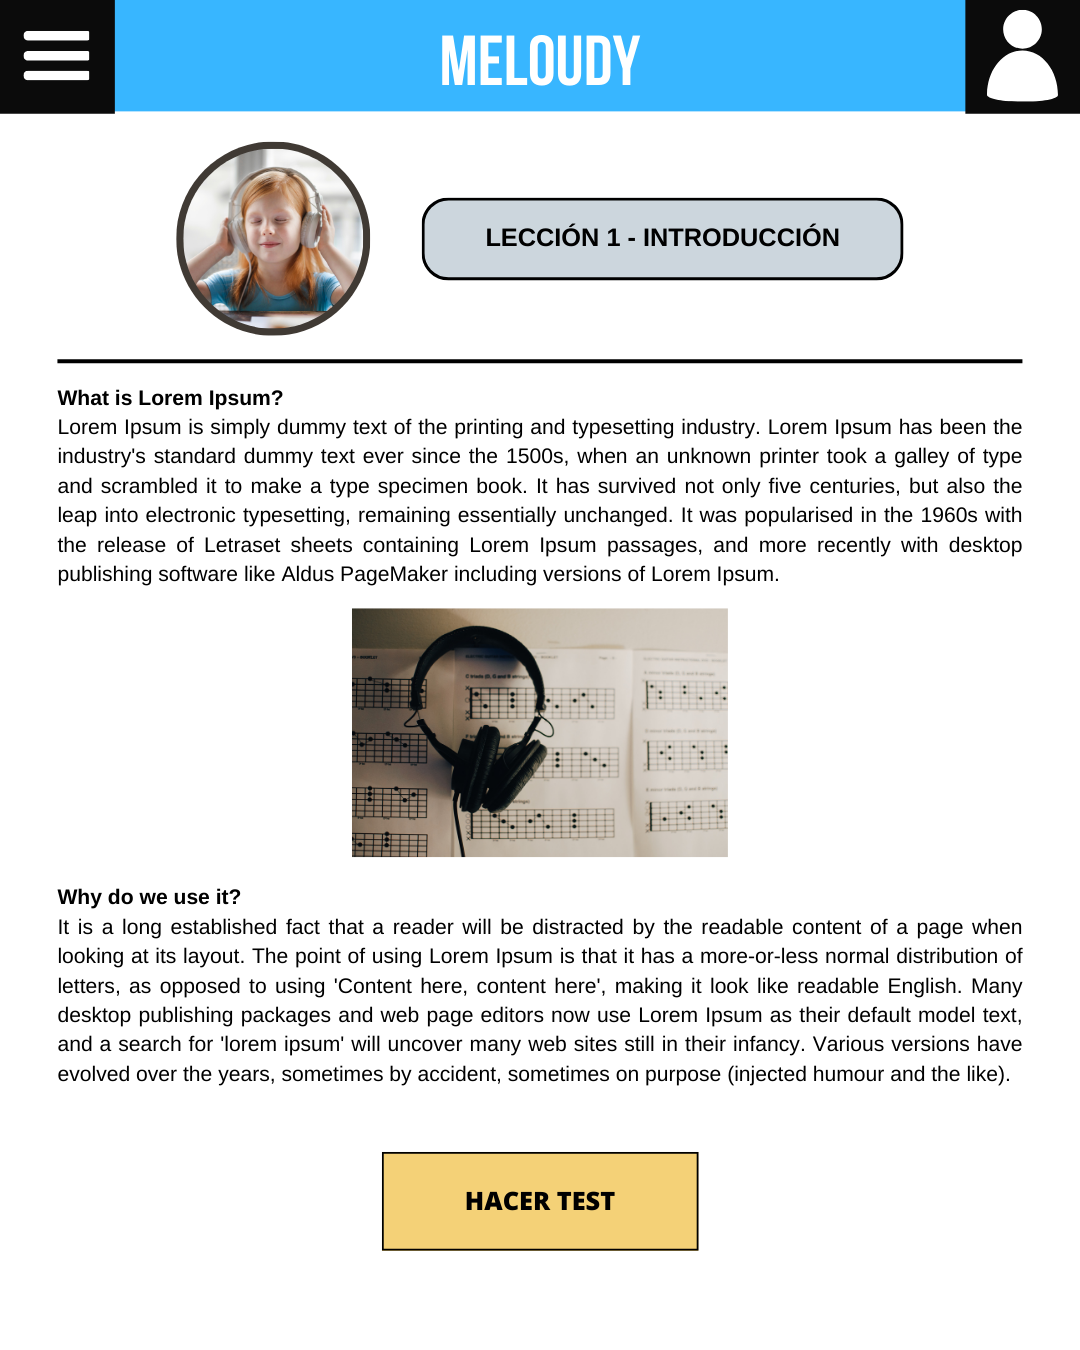
\includegraphics[width=0.55\textwidth, frame]{imagenes/c6/4.png}}
    \caption{Boceto de la pantalla de una lección, con el texto, el contenido multimedia y el botón para comenzar el test.}
    \label{fig:leccion}
\end{figure}

\begin{figure}[H]
    \centering
    \centerline{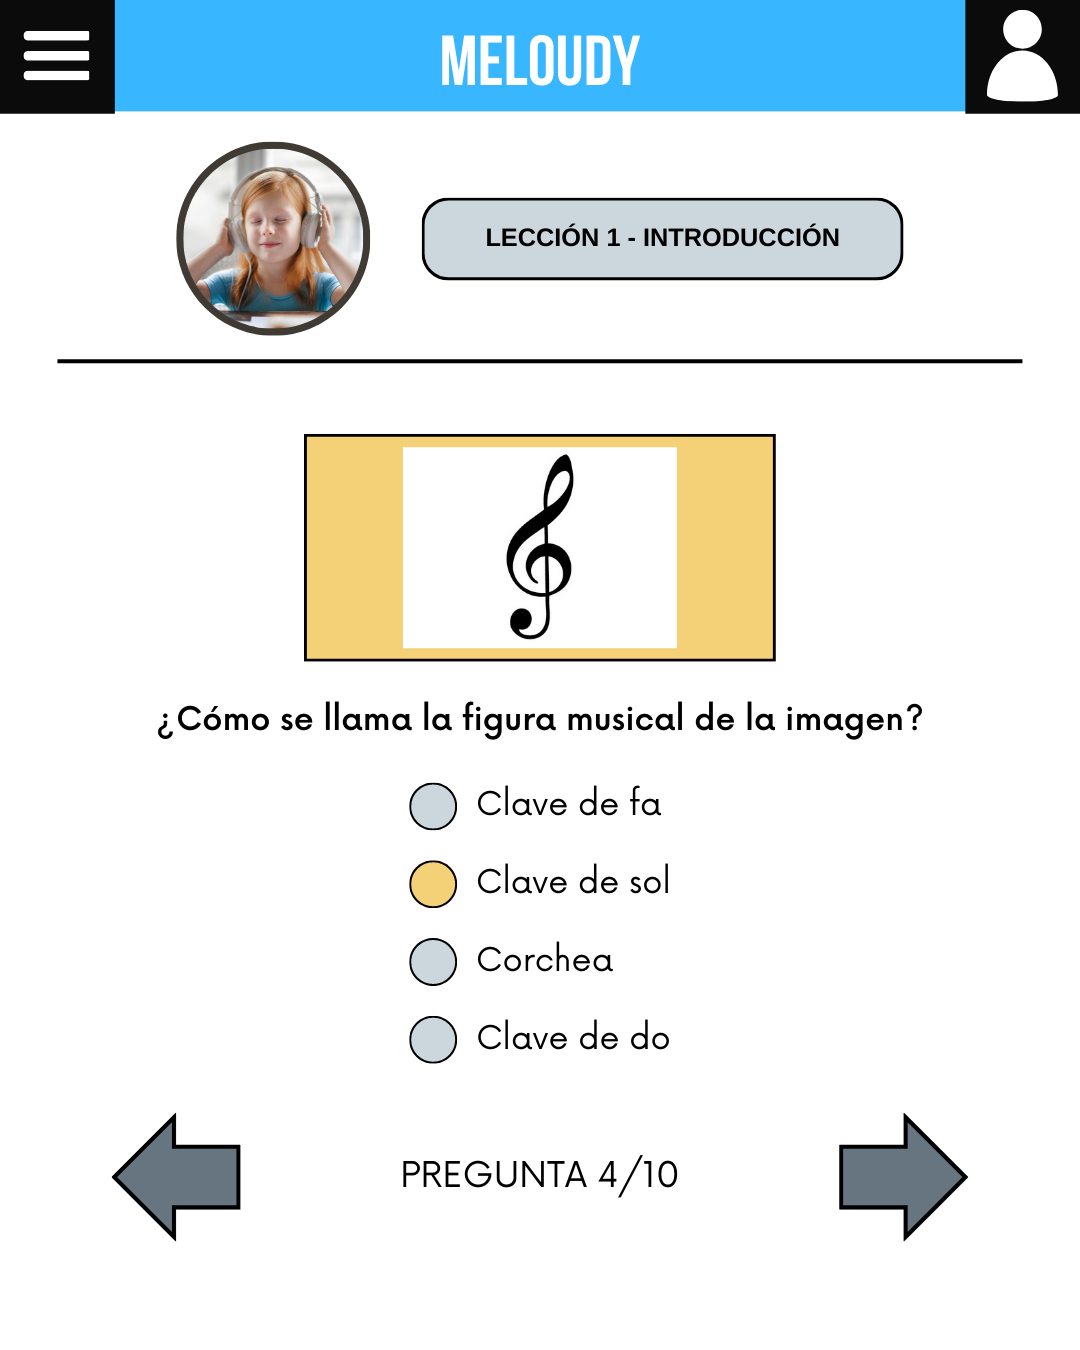
\includegraphics[width=0.55\textwidth, frame]{imagenes/c6/5.png}}
    \caption{Boceto de la pantalla de una pregunta de test de tipo selección única.}
    \label{fig:seleccionunica}
\end{figure}

\begin{figure}[H]
    \centering
    \centerline{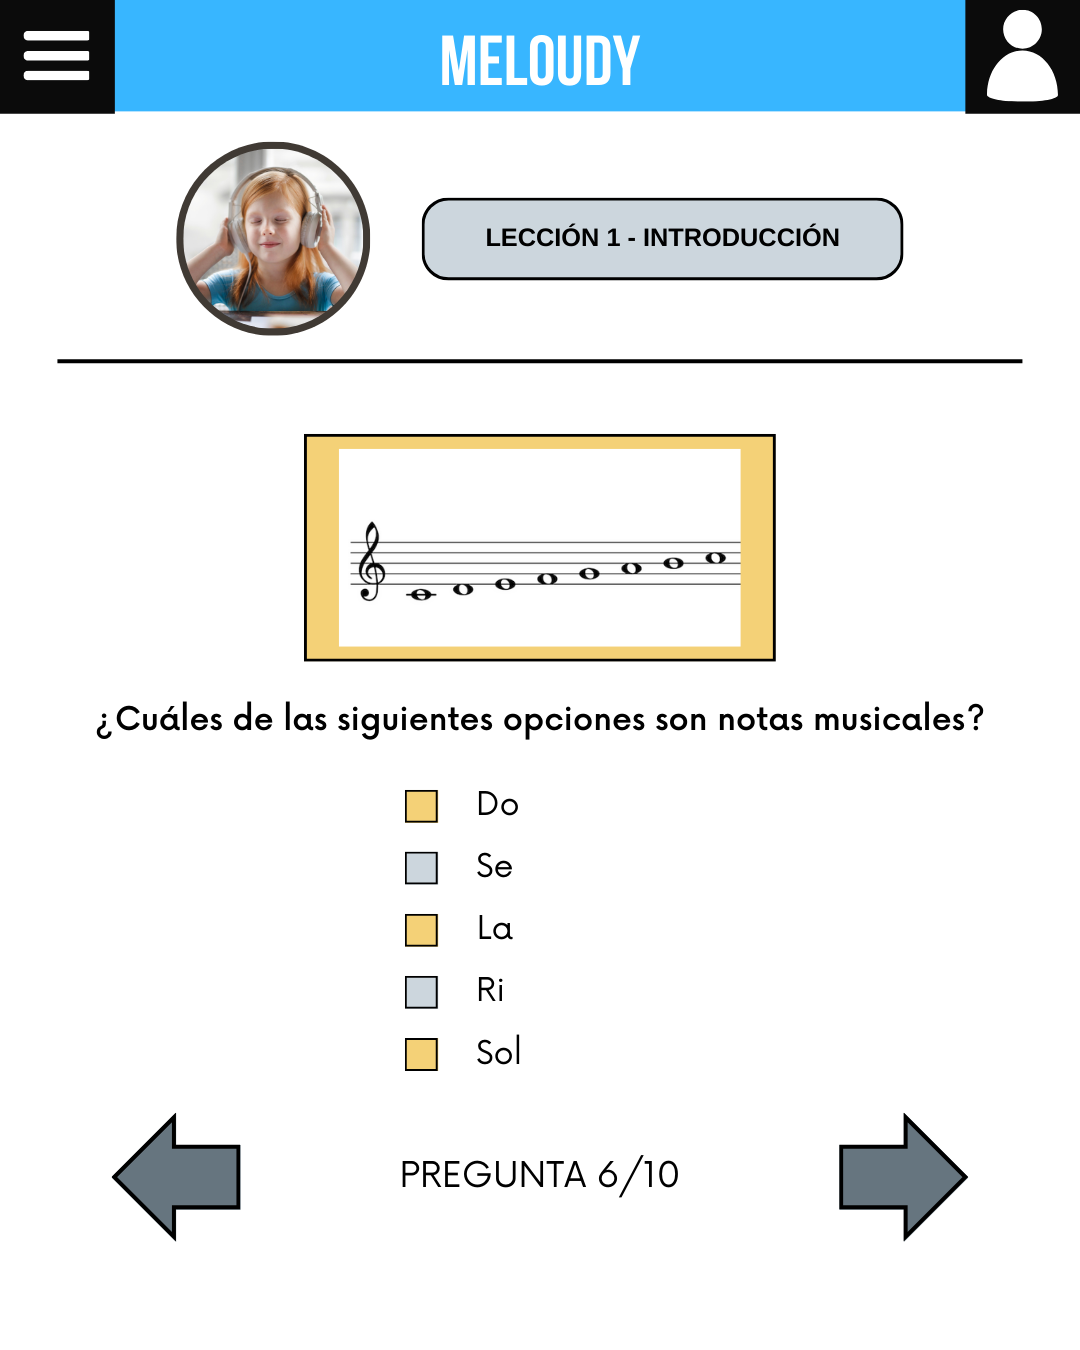
\includegraphics[width=0.55\textwidth, frame]{imagenes/c6/6.png}}
    \caption{Boceto de la pantalla de una pregunta de test de tipo selección multiple.}
    \label{fig:seleccionmultiple}
\end{figure}

\begin{figure}[H]
    \centering
    \centerline{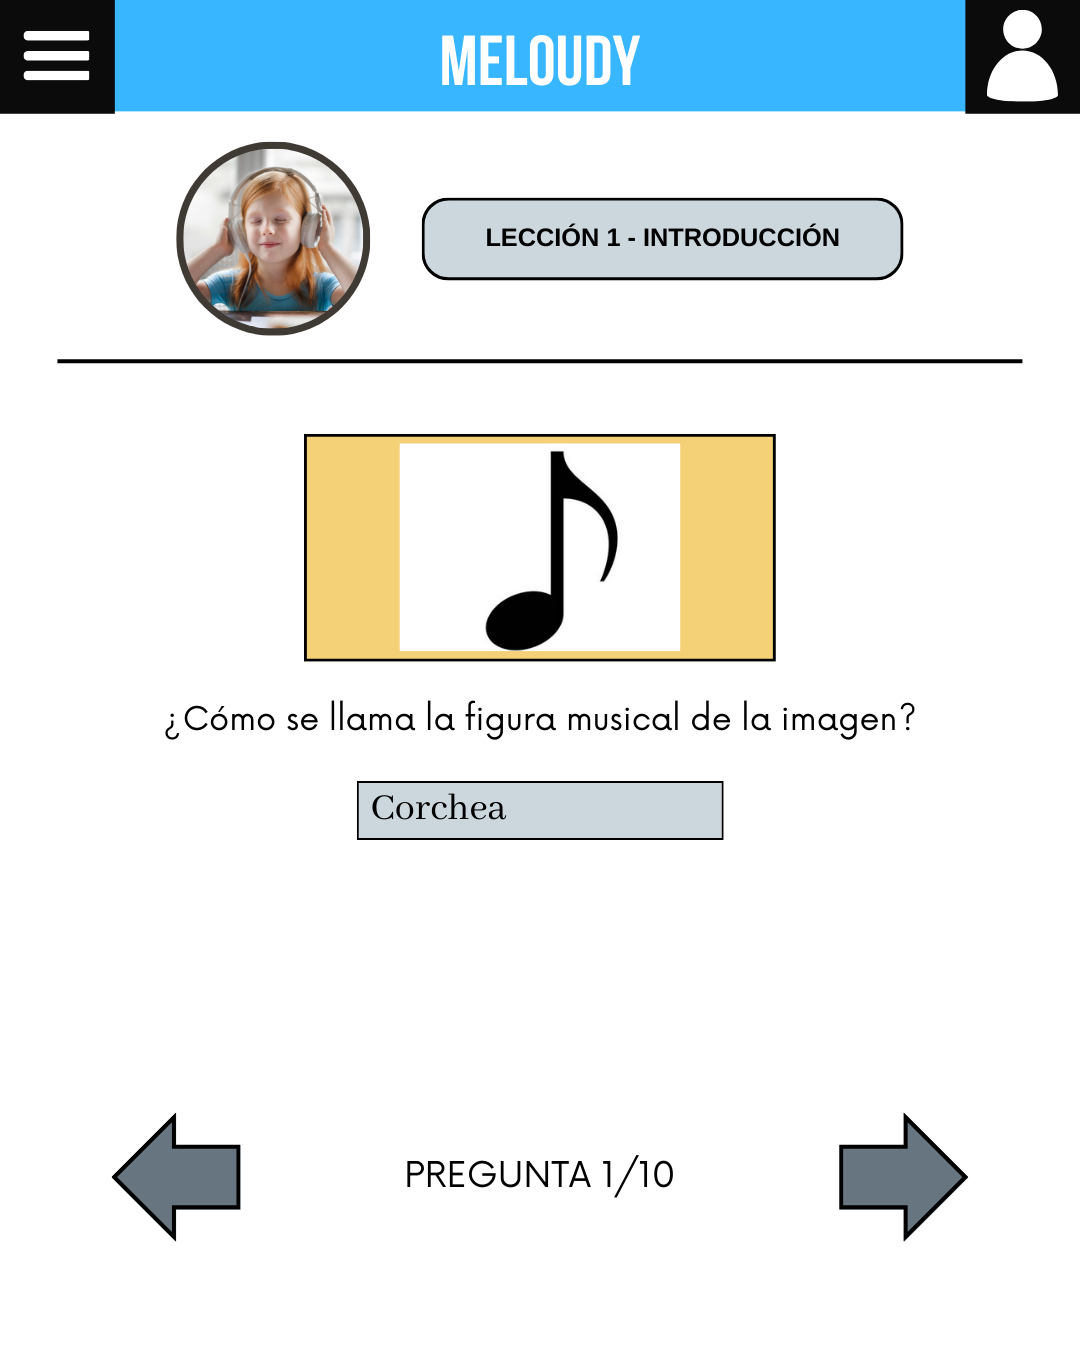
\includegraphics[width=0.55\textwidth, frame]{imagenes/c6/7.png}}
    \caption{Boceto de la pantalla de una pregunta de test de tipo escritura de texto.}
    \label{fig:escrituratexto}
\end{figure}

\begin{figure}[H]
    \centering
    \centerline{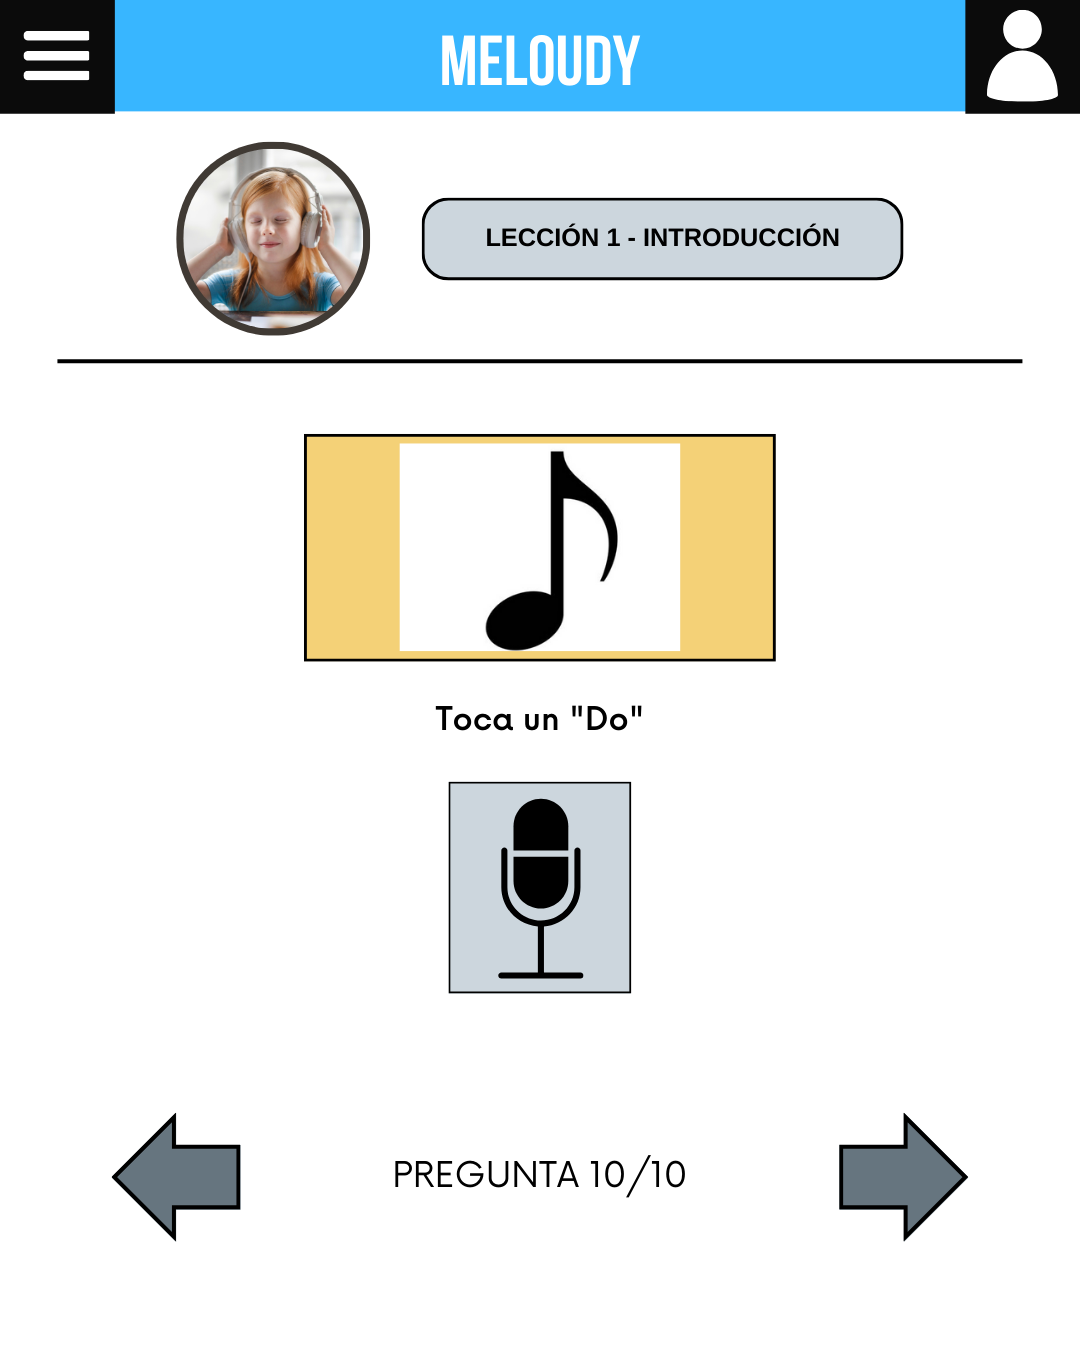
\includegraphics[width=0.55\textwidth, frame]{imagenes/c6/8.png}}
    \caption{Boceto de la pantalla de una pregunta de test de tipo entrada por micrófono.}
    \label{fig:microfono}
\end{figure}

\begin{figure}[H]
    \centering
    \centerline{
\includegraphics[width=0.55\textwidth, frame]{imagenes/c6/9.png}}
    \caption{Boceto de la pantalla de inicio de sesión, donde se pedirá al usuario el correo electrónico y la contraseña.}
    \label{fig:login}
\end{figure}

\begin{figure}[H]
    \centering
    \centerline{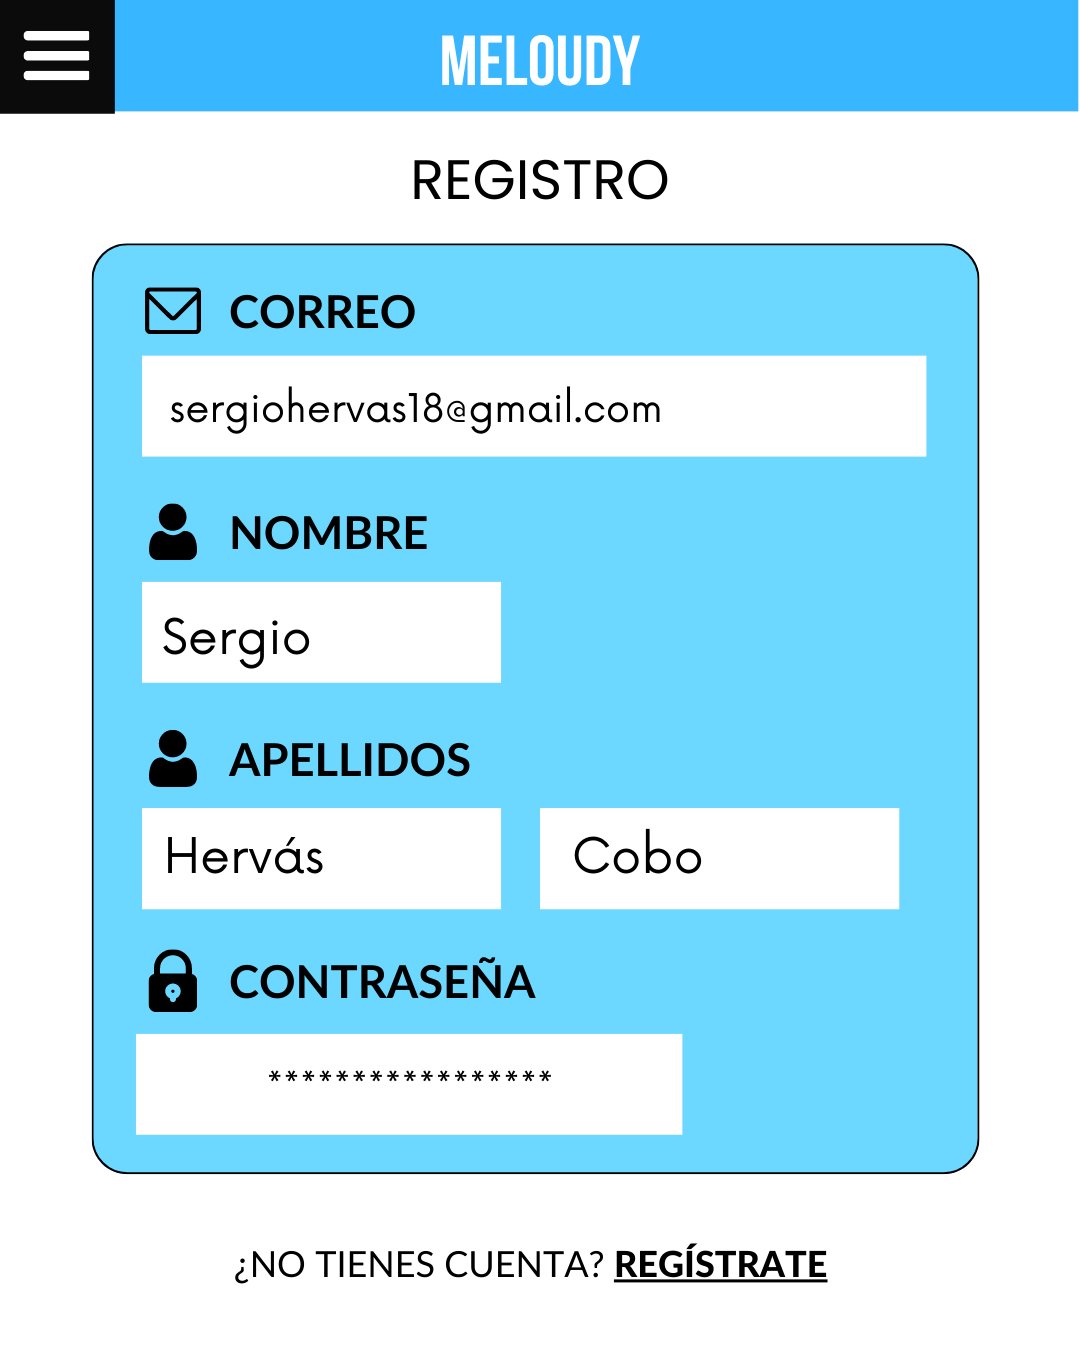
\includegraphics[width=0.55\textwidth, frame]{imagenes/c6/10.png}}
    \caption{Boceto de la pantalla de registro, donde se pedirá al usuario sus datos personales necesarios para crear la cuenta como el nombre, los apellidos, el correo y la contraseña.}
    \label{fig:registro}
\end{figure}